\documentclass[tcc,capa]{texufpel}
\usepackage[utf8]{inputenc}
\usepackage[T1]{fontenc}
\usepackage{lmodern}
\renewcommand{\sfdefault}{phv}
\usepackage{graphicx}
\usepackage{url}
\usepackage{xurl}
\usepackage{array}
\usepackage{booktabs}
\usepackage{longtable}
\usepackage{tabularx}
\usepackage{amsmath}
\newcolumntype{Y}{>{\raggedright\arraybackslash}X}
\usepackage{tikz}
\usetikzlibrary{arrows.meta,positioning,fit,shapes.geometric}
\hypersetup{hidelinks,unicode=true,linktoc=all}

\unidade{Centro de Desenvolvimento Tecnológico}
\curso{Ciência da Computação}
\nomecurso{Bacharelado em Ciência da Computação}
\titulocurso{Bacharel em Ciência da Computação}
\unidadeeng{Technology Development Center}
\cursoeng{Computer Science}
\title{Arquitetura para Gerenciamento Multi-Estruturado de Dados em Sistemas Gamificados: Integração de Fontes Heterogêneas}
\author{Santos}{Rávilon Aguiar dos}
\coadvisor[Prof.~Dr.]{Fleischmann}{Ana Marilza Pernas}
\advisor[Prof.~Dr.]{Ferrugem}{Anderson Priebe}
\keyword{Internet das Coisas;} \keyword{Telemetria;} \keyword{Persistência Poliglota;} \keyword{Gamificação;} \keyword{Eficiência Energética.}
\keywordeng{Internet of Things;} \keywordeng{Telemetry;} \keywordeng{Polyglot Persistence;} \keywordeng{Gamification;} \keywordeng{Energy Efficiency.}

\begin{document}
\renewcommand{\advisorname}{Orientador}
\renewcommand{\coadvisorname}{Coorientadora}
\maketitle
\sloppy
% Substituir por \includepdf{ficha.pdf} após a emissão da ficha no Cobalto.

\begin{abstract}
O projeto de gamificação do Programa de Bom Uso Energético da Universidade Federal de Pelotas busca incentivar mudanças voluntárias de conduta no uso da energia, considerando o conforto dos ocupantes. A previsão de sensores em salas do Centro de Artes e a participação das pessoas em missões exigem uma infraestrutura que integre dados de diferentes origens e mantenha relações entre observações, espaços, usuários e atividades. Este trabalho apresenta o projeto e a implementação da arquitetura de dados e dos serviços desenvolvidos para apoiar o sistema de gamificação associado ao programa. A pesquisa foi organizada segundo a Design Science Research, abordagem de construção e avaliação de artefatos voltados à solução de problemas. O desenvolvimento acompanha o percurso dos dados: recebimento de mensagens de sensores, preservação temporária do conteúdo original, transformação em medições padronizadas, integração de fontes ambientais externas e contexto acadêmico, consulta de agregados e avaliação de condições associadas à gamificação. A solução combina armazenamento documental e relacional por meio de persistência poliglota, conciliando a variabilidade das mensagens com a integridade das relações de domínio. Perfis configuráveis permitem adaptar formatos de sensores, enquanto mecanismos de idempotência e recuperação procuram evitar efeitos repetidos e permitir a retomada do processamento. A versão examinada também contempla fontes compartilhadas de temperatura externa e regras de ambiente que relacionam medições locais, condições temporais e beneficiários. A avaliação distingue a inspeção do código atual dos relatórios históricos de execução e do experimento de comparação de motores de regras. As evidências identificadas sustentam a presença dos mecanismos projetados e delimitam os cenários de verificação, sem transferir resultados antigos para a versão atual. A contribuição é uma base de integração rastreável de fontes heterogêneas, preparada para apoiar análises e futuras intervenções gamificadas no contexto institucional.
\end{abstract}

\begin{englishabstract}{Architecture for Multi-Structured Data Management in Gamified Systems: Integration of Heterogeneous Data Sources}
The gamification project of the energy-use program at the Federal University of Pelotas aims to encourage voluntary changes in energy-use behavior while considering occupant comfort. Planned sensors in rooms at the Center for Arts and people's participation in missions require infrastructure that integrates heterogeneous sources and relates observations, spaces, users, and activities. This work presents the design and implementation of the data architecture and supporting services developed for the institutional gamification system. Design Science Research guided artifact development and evaluation. The presentation follows the data lifecycle: receiving sensor messages, temporarily preserving original content, transforming it into standardized measurements, integrating external environmental sources and academic context, querying aggregates, and evaluating conditions associated with gamification. The solution combines document and relational storage through polyglot persistence, accommodating variable messages and structured domain relationships. Configurable integration profiles support different sensor formats, while idempotency and recovery mechanisms address repeated effects and interrupted processing. The examined version also includes shared outdoor-temperature sources and environmental rules that relate local measurements, temporal conditions, and beneficiaries. Evaluation distinguishes inspection of the current source code from historical execution reports and a rule-engine comparison experiment. The identified evidence supports the presence of the designed mechanisms and defines the examined verification scenarios without transferring earlier results to the current version. The contribution is traceable integration infrastructure for heterogeneous sources, intended to support analysis and future institutional gamification interventions.
\end{englishabstract}

\listoffigures
\listoftables
\begin{listofabbrv}{PROBEN}
\item[\textbf{API}] Application Programming Interface
\item[\textbf{DSR}] Design Science Research
\item[\textbf{HTTP}] Hypertext Transfer Protocol
\item[\textbf{IoT}] Internet of Things
\item[\textbf{JSON}] JavaScript Object Notation
\item[\textbf{JWT}] JSON Web Token
\item[\textbf{MQTT}] MQTT --- protocolo de publicação e assinatura de mensagens
\item[\textbf{PROBEN}] Programa de Bom Uso Energético
\item[\textbf{QoS}] Quality of Service
\item[\textbf{REST}] Representational State Transfer
\item[\textbf{TTL}] Time to Live
\item[\textbf{UFPel}] Universidade Federal de Pelotas
\item[\textbf{XP}] Experience Points
\end{listofabbrv}
\tableofcontents

\chapter{Introdução}\label{cap:introducao}
O uso consciente da energia em uma edificação depende tanto de suas instalações quanto das práticas de quem a ocupa. A gamificação pode apoiar intervenções nesse contexto ao associar informações sobre consumo a metas, participação e retorno aos usuários. Estudos em escritórios ilustram essa possibilidade, mas também mostram que o desenho e a avaliação da intervenção precisam considerar o ambiente e seus participantes \cite{oppong2020,iria2020}. Para que uma intervenção assim seja viável, existe uma questão anterior: como reunir dados ambientais e registros de participação de forma que possam ser interpretados em conjunto?

Na Universidade Federal de Pelotas (UFPel), o Programa de Bom Uso Energético (PROBEN) articula ações de educação e gestão energética \cite{probenUfpel2026}. Nesse contexto, o projeto ``Validação de sistema de gamificação, gestão e automação na nuvem para eficiência energética de edificações públicas com foco inicial em universidades'' prevê o uso de software para apoiar mudanças voluntárias de conduta. A proposta institucional abrange desenvolvimento, validação e avaliação de engajamento e consumo.\footnote{Descrição institucional do projeto fornecida pelo autor durante a revisão do TCC. As metas do projeto institucional delimitam o contexto; não constituem resultados obtidos pelo sistema.} Este trabalho se insere nessa iniciativa e trata da infraestrutura de dados necessária à futura aplicação de gamificação.

O cenário inicial é o Centro de Artes da UFPel, em cujas salas está prevista a disponibilização de sensores. As observações produzidas por esses dispositivos precisam ser relacionadas aos espaços, às condições externas, aos horários de uso e às pessoas que participam das atividades. O objetivo institucional é incentivar hábitos de uso consciente da energia, considerando o conforto, e não apenas acumular leituras. A integração dos dados constitui, portanto, uma condição para que regras e missões possam fazer sentido no contexto em que serão aplicadas.

\section{Do cenário institucional ao problema de dados}
Uma leitura de temperatura, isoladamente, informa pouco sobre uma ação de eficiência energética. Para interpretá-la, pode ser necessário saber em qual sala foi obtida, quando ocorreu, se há atividade prevista naquele local, quais pessoas são elegíveis à atividade e qual condição ambiental externa serve de referência. A relevância do contexto na interpretação de observações técnicas e humanas é discutida por Sagl, Resch e Blaschke \cite{sagl2015}. No presente trabalho, essa relação é concretizada por vínculos entre medições, salas, dados acadêmicos, participação e regras configuráveis.

A diversidade das entradas acrescenta outro desafio. Modelos de sensores podem transmitir a mesma grandeza com nomes de campos e estruturas diferentes. Um dispositivo pode ser substituído durante a operação; uma fonte meteorológica pode atender várias salas; e uma mensagem pode chegar novamente após uma falha de comunicação. A infraestrutura precisa absorver essas diferenças sem transformar cada troca de dispositivo em uma mudança de toda a modelagem. Também deve evitar que a repetição de uma mensagem gere uma nova medição ou que a repetição do processamento gere uma nova recompensa.

As pessoas constituem outra origem de registros. A adesão a uma missão, a confirmação de presença e o progresso de uma atividade são dados de participação, distintos de observações físicas. A aplicação móvel que produzirá parte dessas interações é uma consumidora futura dos serviços desenvolvidos. O artefato deste TCC implementa a base para recebê-las e relacioná-las, sem incluir o desenvolvimento do cliente móvel nem a avaliação de mudanças comportamentais.

O título deste trabalho expressa esse recorte. ``Arquitetura para gerenciamento multi-estruturado de dados'' designa a organização dos mecanismos que integram mensagens documentais, entidades relacionais, séries de medições e registros de gamificação. ``Sistemas gamificados'' identifica o domínio no qual esses dados dão suporte à participação e às atividades dos usuários. ``Fontes heterogêneas'' abrange as diferenças de origem, estrutura e significado entre sensores, serviços externos e registros das pessoas.

\section{Questão de pesquisa e objetivos}
A questão investigada é: \emph{como projetar uma infraestrutura de dados que integre observações ambientais heterogêneas e registros de participação, preserve sua rastreabilidade e sustente análises e mecanismos de gamificação da eficiência energética?}

O objetivo geral é projetar, implementar e examinar uma arquitetura de dados e serviços que responda a essa questão no contexto do PROBEN. Os objetivos específicos são:
\begin{enumerate}
\item caracterizar as fontes e as relações entre sensores, espaços, pessoas e atividades;
\item estabelecer formas de preservar mensagens originais e representar medições padronizadas;
\item implementar comunicação por Hypertext Transfer Protocol (HTTP), por requisição e resposta, e por MQTT, com publicação e assinatura de mensagens, tratando repetição e conflito;
\item permitir a configuração de formatos e modelos de sensores por perfis de integração;
\item integrar fontes ambientais compartilhadas e informações acadêmicas à interpretação das medições;
\item oferecer interfaces de consulta e administração, agregação temporal e avaliação de missões e regras de ambiente;
\item relacionar evidências, atividades e pontos com mecanismos de idempotência e recuperação;
\item examinar as decisões por inspeção do artefato, cenários de testes e análise crítica das evidências de execução disponíveis.
\end{enumerate}

\section{Escopo, contribuição e organização}
A contribuição é uma infraestrutura em que formatos de entrada podem variar, enquanto as relações necessárias à análise e à gamificação permanecem explicitamente modeladas. O trabalho articula persistência poliglota, integração configurável, contexto compartilhado e processamento rastreável. A possibilidade de expansão institucional orienta essas decisões, mas sua comprovação exige medições de carga e operação em outros ambientes.

A avaliação se concentra nas propriedades do software. Economia de energia, adesão sustentada e conforto percebido dependem de uma intervenção posterior com ocupantes e instrumentos de medição apropriados. Essa separação mantém a contribuição verificável e evita tomar a existência de pontos ou de uma condição térmica calculada como comprovação de benefício ambiental.

O Capítulo~\ref{cap:fundamentos} apresenta os conceitos necessários para acompanhar o percurso dos dados. O Capítulo~\ref{cap:relacionados} relaciona esses conceitos a estudos de integração e gamificação. O Capítulo~\ref{cap:metodo} descreve o método e as fontes de evidência. O Capítulo~\ref{cap:desenvolvimento} acompanha os dados da origem ao uso, explicitando desafios e decisões. O Capítulo~\ref{cap:avaliacao} examina o alcance das evidências, e o Capítulo~\ref{cap:conclusao} sintetiza a contribuição e suas possibilidades de continuidade.

\chapter{Fundamentação Teórica}\label{cap:fundamentos}
O problema investigado reúne três necessidades: interpretar observações de origens distintas, armazená-las segundo suas características e utilizá-las em decisões contextualizadas. Este capítulo apresenta os conceitos que dão suporte a essas necessidades. A discussão parte das fontes, passa por comunicação e persistência e chega ao tratamento temporal e ao uso das informações em gamificação.

\section{Observações ambientais e participação humana}
\emph{Internet of Things} (IoT), ou Internet das Coisas, relaciona objetos físicos, sensoriamento e comunicação para disponibilizar observações e serviços. Gubbi et al. \cite{gubbi2013} e Al-Fuqaha et al. \cite{alfuqaha2015} discutem seus elementos arquiteturais e tecnologias de comunicação. Para este TCC, o ponto relevante é a separação entre a grandeza observada e a maneira como cada dispositivo a transmite.

O valor de uma observação depende de contexto espacial, temporal e de sua origem. Sagl, Resch e Blaschke \cite{sagl2015} discutem a integração de informações produzidas por sensores técnicos e por pessoas. Essa perspectiva sustenta a inclusão de registros humanos como fonte complementar, preservando sua natureza: uma pessoa declarar participação não equivale a um sensor medir energia. Na infraestrutura desenvolvida, a distinção orienta a modelagem de presença, adesão, atividade e medição.

\section{Comunicação e interpretação de formatos}
\emph{Hypertext Transfer Protocol} (HTTP) é um protocolo de aplicação baseado em requisições e respostas. Ele permite que clientes submetam dados e consultem recursos em um servidor \cite{http2022}. \emph{Application Programming Interface} (API) é a interface por meio da qual uma aplicação disponibiliza operações a outras. No trabalho, a API oferece os serviços de recebimento, configuração e consulta.

\emph{Representational State Transfer} (REST) é um estilo arquitetural definido por restrições como separação entre cliente e servidor, comunicação sem estado de sessão no servidor e interface uniforme \cite{fielding2000}. Assim, HTTP é o protocolo empregado e REST descreve uma orientação de organização das interfaces. O emprego de rotas HTTP, por si só, não demonstra atendimento integral a todas as restrições REST.

MQTT é um protocolo de mensageria baseado em publicação e assinatura. Um produtor publica mensagens em tópicos de um intermediário, o \emph{broker}, e consumidores recebem as mensagens dos tópicos assinados. A especificação define níveis de \emph{Quality of Service} (QoS), isto é, qualidade do serviço de entrega. Em QoS~1, a entrega é de pelo menos uma vez e admite duplicatas \cite{oasisMqtt2019}. Essa garantia de transporte não demonstra a conclusão das operações de domínio, como registrar uma medição ou atribuir pontos.

O formato dos dados constitui uma dimensão diferente do protocolo. \emph{JavaScript Object Notation} (JSON) é um formato textual de representação de dados \cite{json2017}. Dois produtores podem usar JSON e ainda assim representar temperatura em campos diferentes. A transformação para uma representação comum, denominada modelo canônico neste trabalho, procura estabilizar a interpretação usada pelas etapas seguintes. Sua realização depende de identificadores, tipos, unidades e mapeamentos explícitos, e não apenas da adoção do mesmo protocolo.

\section{Persistência poliglota e integridade}
\emph{Polyglot persistence}, ou persistência poliglota, corresponde ao uso de diferentes mecanismos de armazenamento para diferentes finalidades em uma mesma aplicação. Grolinger et al. \cite{grolinger2013} discutem explicitamente o conceito ao revisar bancos não relacionais e suas possibilidades de uso. Gessert et al. \cite{gessert2017} relacionam a escolha de armazenamento aos requisitos funcionais e não funcionais. Esses estudos permitem fundamentar a escolha pelos dados e operações esperados.

No problema deste TCC, mensagens originais podem ter estruturas variáveis e precisam permanecer disponíveis para inspeção e nova interpretação durante um período. Pessoas, salas, medições, regras e recompensas, por sua vez, estabelecem relações que exigem integridade. Essa diferença motiva a combinação entre armazenamento documental e relacional. Não decorre, entretanto, que um banco relacional seja incapaz de guardar documentos, nem que dois bancos sejam necessariamente superiores a um. A decisão introduz o custo adicional de coordenar estados e preservar referências entre os armazenamentos.

\section{Tempo, repetição e recuperação do processamento}
O instante em que uma observação ocorre pode diferir daquele em que é recebida ou processada. Akidau et al. \cite{akidau2015} mostram a importância dessa distinção para fluxos não limitados e fora de ordem, relacionando tempo do evento, janelas e resultados. Neste trabalho, essas ideias fundamentam a necessidade de explicitar intervalos e políticas de atraso; não implicam adoção integral do modelo Dataflow.

Idempotência significa que repetir uma operação não multiplica seu efeito esperado. A semântica de métodos idempotentes é descrita para HTTP em sua especificação \cite{http2022}; no PROBEN, a propriedade também é implementada no domínio por identidades e restrições de unicidade. Uma tentativa repetida com o mesmo conteúdo pode ser reconhecida; conteúdo diferente sob a mesma identidade deve ser tratado como conflito.

Um processamento assíncrono também precisa distinguir trabalho reservado de trabalho concluído. Neste texto, \emph{claim} designa a reserva atômica de um item e \emph{lease}, a concessão temporária dessa reserva. Ao expirar, ela permite a retomada por outro executor. São mecanismos concretos do artefato, cuja implementação e cenários de verificação serão discutidos adiante; sua presença não garante recuperação sob qualquer falha distribuída.

\section{Gamificação e uso consciente da energia}
Gamificação utiliza elementos de projeto de jogos em contextos que não são jogos \cite{deterding2011}. No domínio energético, ela pode combinar metas, retorno sobre comportamento e participação. Morschheuser et al. \cite{morschheuser2018} propõem um método de desenvolvimento que considera análise do contexto e avaliação iterativa. Oppong-Tawiah et al. \cite{oppong2020} exemplificam essa relação em uma aplicação voltada a práticas sustentáveis no escritório.

Para o PROBEN, a relevância está em permitir que uma atividade seja contextualizada e que o participante compreenda o retorno recebido. Pontos são uma representação de progresso, não uma medida física de energia. O projeto institucional pretende favorecer mudanças voluntárias de conduta; o presente artefato fornece os serviços e registros para essa intervenção, mantendo separadas as condições de avaliação técnica e as de avaliação comportamental.

\section{Conforto térmico adaptativo como requisito de contexto}
O conforto térmico adaptativo relaciona condições internas às expectativas e à experiência térmica dos ocupantes. De Dear e Brager \cite{deDear2002} apresentam resultados e uma proposta para ambientes naturalmente ventilados, ressaltando o papel das condições externas. Esse fundamento explica por que a temperatura externa pode ser relevante para interpretar uma sala, além da medição interna.

O conceito não autoriza aplicar uma mesma equação indistintamente a qualquer ambiente climatizado. Para o TCC, importa distinguir a hipótese de domínio, a regra calculada no software e a avaliação real do conforto. O primeiro aspecto é fundamentado na literatura; o segundo depende da implementação e dos dados; o terceiro requer critérios de aplicabilidade e estudo de campo. A infraestrutura desenvolvida atua principalmente no segundo aspecto.

\chapter{Trabalhos Relacionados}\label{cap:relacionados}
A literatura pertinente ao trabalho pode ser organizada em duas perspectivas complementares: intervenções que utilizam dados para incentivar comportamentos e soluções que tratam a integração e o processamento desses dados. Esta comparação procura identificar o que cada perspectiva informa à construção do artefato, sem supor que estudos com objetivos diferentes devam apresentar os mesmos mecanismos técnicos.

\section{Dados e participação em intervenções energéticas}
Orland et al. \cite{orland2014} investigam uma intervenção com jogo em ambiente de escritório, conectando consumo monitorado e participação. Sua relevância para este TCC é a associação entre evidências do ambiente e retorno aos usuários. Os resultados de uma intervenção concreta dependem das cargas e dos participantes estudados, não sendo uma previsão de economia para outra plataforma.

Oppong-Tawiah et al. \cite{oppong2020} descrevem o desenvolvimento de uma aplicação móvel em cinco ciclos de projeto, combinando acompanhamento de uso de eletricidade e estratégias de engajamento. A relação mais direta com este trabalho é a necessidade de articular construção do sistema e avaliação. O objeto aqui delimitado, contudo, é a infraestrutura de dados que antecede a intervenção móvel.

Iria et al. \cite{iria2020} apresentam uma plataforma para eficiência energética em escritórios que utiliza informação de contexto, painéis e estratégias de participação. A comparação destaca o papel da informação ambiental na comunicação com o usuário. Neste TCC, essa necessidade leva a representar explicitamente fontes locais e externas e os vínculos entre dados e decisões.

Esses trabalhos fundamentam a relevância de integrar medição e participação. Eles não fornecem, apenas pela descrição desses mecanismos, evidência de que o PROBEN evita duplicatas ou recupera uma tarefa interrompida. Essas propriedades precisam ser examinadas no artefato desenvolvido.

\section{Representação e processamento dos dados}
Grolinger et al. \cite{grolinger2013} fornecem uma visão das possibilidades e desafios de bancos com diferentes modelos. Gessert et al. \cite{gessert2017} apresentam orientação de seleção conforme requisitos. Sua contribuição ao TCC está em deslocar a decisão de armazenamento do nome da tecnologia para as operações necessárias. O artefato utiliza essa perspectiva para separar preservação documental e relações de domínio, assumindo o custo de integração entre elas.

Akidau et al. \cite{akidau2015} abordam o processamento de dados não limitados e fora de ordem, discutindo compromissos entre correção, latência e custo. A arquitetura desenvolvida emprega uma solução mais restrita: janelas persistidas, agregação de medições existentes e recomputação explícita. A comparação torna visíveis tanto a inspiração conceitual quanto a ausência de mecanismos mais amplos de atualização automática de resultados diante de atrasos.

\begin{table}[htbp]\centering\small
\caption{Relação entre a literatura e o problema investigado}\label{tab:relacionados}
\begin{tabularx}{\textwidth}{p{3.1cm}YY}\toprule
Estudo & Contribuição utilizada & Delimitação no TCC \\\midrule
Orland et al.; Iria et al. & Relação entre informação ambiental e intervenção gamificada. & Infraestrutura de dados; efeitos comportamentais não avaliados. \\
Oppong-Tawiah et al. & Desenvolvimento e avaliação iterativos em sustentabilidade. & Artefato de integração, sem cliente móvel. \\
Grolinger et al.; Gessert et al. & Escolha de armazenamento conforme os requisitos. & Combinação documental e relacional, sem comparação experimental entre bancos. \\
Akidau et al. & Tempo do evento, janelas e dados fora de ordem. & Janelas e recuperação persistidas, com política limitada de recomputação. \\\bottomrule
\end{tabularx}
\caption*{Fonte: síntese do autor a partir dos estudos citados no capítulo.}
\end{table}

\section{Posicionamento da contribuição}
A Tabela~\ref{tab:relacionados} mostra que a contribuição pretendida não é uma nova teoria de motivação nem um novo banco de dados. Ela está na articulação de mecanismos de integração em um problema institucional: permitir que uma observação heterogênea seja preservada, interpretada, contextualizada e relacionada a efeitos de gamificação de forma inspecionável. Trata-se de uma contribuição aplicada de projeto e desenvolvimento, cujo alcance depende da evidência apresentada para cada propriedade.

\chapter{Metodologia}\label{cap:metodo}
A organização da pesquisa procura relacionar o problema institucional às decisões de construção e à avaliação do artefato. Este capítulo explicita essa relação e define como interpretar as evidências utilizadas, distinguindo inspeção da implementação, cenários de teste e resultados de execuções anteriores.

\section{Abordagem de pesquisa}
O trabalho adota \emph{Design Science Research} (DSR), abordagem em que a construção e avaliação de artefatos se relacionam a problemas relevantes \cite{hevner2004}. As atividades de identificação do problema, definição de objetivos, desenvolvimento, demonstração, avaliação e comunicação seguem a organização de Peffers et al. \cite{peffers2007}. A aplicação do método ao TCC é apresentada na Tabela~\ref{tab:metodo}.

\begin{table}[htbp]\centering\small
\caption{Atividades de pesquisa e sua realização no trabalho}\label{tab:metodo}
\begin{tabularx}{\textwidth}{p{3.4cm}Y}\toprule
Atividade & Realização e produto \\\midrule
Identificar o problema & Caracterização do cenário, das fontes e dos riscos de integrar observações e participação. \\
Definir objetivos & Formulação dos requisitos de integração, integridade, contexto e rastreabilidade. \\
Projetar e desenvolver & Construção incremental de recebimento, representação comum, fontes compartilhadas, consultas, missões e regras de ambiente. \\
Demonstrar & Exemplos de percurso dos dados, cenários automatizados e registros operacionais disponíveis. \\
Avaliar & Confronto entre requisito, mecanismo implementado, cenário de teste e evidência de execução. \\
Comunicar & Texto do TCC, figuras, documentação técnica e referências versionadas. \\\bottomrule
\end{tabularx}
\caption*{Fonte: elaboração do autor.}
\end{table}

Os requisitos foram reconstruídos a partir do escopo institucional, das discussões de desenvolvimento e da evolução documentada do sistema. Não foi realizado um protocolo formal de entrevistas com usuários finais. O histórico auxilia a explicar as necessidades, mas não permite afirmar que todas as alternativas foram comparadas experimentalmente. Quando uma decisão é discutida por suas vantagens e custos, trata-se de análise do projeto; a existência de um experimento é indicada separadamente.

\section{Requisitos e critérios de observação}
O conjunto da Tabela~\ref{tab:requisitos} preserva os objetivos de recebimento, transformação, análise e gamificação e incorpora as necessidades de fontes externas e regras de ambiente da versão atual. A numeração organiza a argumentação deste TCC; não corresponde a um catálogo histórico de requisitos aprovado em uma única etapa.

\begin{table}[htbp]\centering\small
\caption{Requisitos utilizados para orientar a análise do artefato}\label{tab:requisitos}
\begin{tabularx}{\textwidth}{p{0.7cm}p{3.2cm}Y}\toprule
Id. & Necessidade & Critério observável \\\midrule
R1 & Receber fontes diversas & Entradas HTTP e MQTT, identificação de origem e tratamento de formatos. \\
R2 & Preservar e reinterpretar & Conteúdo bruto temporário, histórico e vínculo com a medição resultante. \\
R3 & Evitar efeitos repetidos & Unicidade e distinção entre repetição equivalente e conflito. \\
R4 & Adaptar modelos de sensores & Tipos, parâmetros e perfis de integração configuráveis. \\
R5 & Contextualizar observações & Relações com salas, fontes compartilhadas, horários e pessoas. \\
R6 & Analisar períodos & Janelas definidas, agregados consultáveis e política de recomputação. \\
R7 & Apoiar gamificação & Evidências, ocorrências, atividades e pontos relacionados. \\
R8 & Recuperar processamento & Estados persistidos, reserva temporária e controle de concorrência. \\
R9 & Administrar e proteger & Console, autenticação e autorização de operações. \\
R10 & Avaliar o ambiente & Regras locais e padrões, dados válidos, contexto e beneficiários. \\\bottomrule
\end{tabularx}
\caption*{Fonte: elaboração do autor.}
\end{table}

\section{Versões e fontes de evidência}\label{sec:versoes}
A descrição atual da arquitetura está vinculada ao commit \path{5e2a1e27d2f4ceb31217867259a303eee84b3c0f}, consultado em 12 de novembro de 2026, do repositório \path{ravilon/PROCEL-Back-End}. Os módulos dessa versão são \path{Proben-API}, \path{Proben-Telemetry} e \path{Proben-Admin}, identificadores históricos que correspondem, respectivamente, ao serviço de integração, processamento e disponibilização de dados, ao serviço de coleta e persistência de dados brutos e à interface de administração e configuração. Essas denominações funcionais são empregadas ao longo do texto; os nomes de implementação permanecem onde a reprodução técnica os exige. Foram inspecionados código de serviços, cenários de testes, migrations de fontes compartilhadas e regras de ambiente, além dos documentos técnicos indicados no Apêndice~\ref{ap:evidencias} \cite{probenAtual2026}.

A inspeção examina o que está implementado e quais oráculos os testes expressam. A etapa atual de avaliação não inclui uma nova execução das suítes Java ou do console web. Portanto, a presença de um teste não é apresentada como aprovação do caso. O relatório operacional de setembro e os números do experimento de motores são tratados como evidências históricas, com o alcance de suas próprias fontes. A versão histórica anteriormente utilizada no TCC, \path{141db8ccbf63cf3896344fbb90197dfae3618691}, é mantida nas referências históricas e não substituída pelo hash atual \cite{probenReadme2026,probenSmoke2026,probenDrools2026}.

Essa separação é necessária porque atualizar o texto de uma funcionalidade não atualiza os resultados de seu teste. Contagens de classes, migrations ou anotações de teste também não demonstram correção. A análise utiliza a cadeia requisito--mecanismo--cenário--evidência, indicando onde existe apenas inspeção, onde há registro de execução anterior e onde permanece uma lacuna.

\section{Seleção de literatura e tratamento dos termos}
A revisão de literatura é narrativa, orientada pela relação entre conceito e decisão de projeto. Foram priorizados artigos revisados por pares e fontes originais, com verificação de título, autoria e identificador digital quando disponível. Trabalhos sobre integração, armazenamento, fluxos, gamificação e conforto foram utilizados segundo o aspecto que efetivamente sustentam. Normas e especificações fundamentam protocolos e formatos; documentação do sistema fundamenta o comportamento implementado.

A reputação e a classificação dos veículos são critérios auxiliares, não substitutos da leitura. Não se atribuem estratos Qualis sem consulta identificada de periódico e período. A CAPES esclarece que o Qualis Periódicos 2021--2024 tem finalidade e período específicos e não será atualizado para o ciclo 2025--2028 \cite{capes2026}. Nesta revisão não foi concluída uma classificação individual dos veículos; assim, não se afirma que todas as referências pertencem a determinado estrato. A matriz de referências e verificações acompanha o texto no repositório do TCC.

Termos em português são empregados quando consolidados. Nos demais casos, mantém-se a expressão original e apresenta-se sua função em português. Siglas são definidas na primeira ocorrência pertinente. Essa escolha busca permitir que o argumento seja compreendido sem exigir familiaridade prévia com os nomes de componentes de software.

\chapter{Da Origem dos Dados ao Apoio à Gamificação}\label{cap:desenvolvimento}
A arquitetura é apresentada neste capítulo pelo percurso dos dados. Primeiro são identificadas suas origens e os espaços aos quais se referem. Em seguida, são discutidos recebimento, preservação, transformação e contextualização. Finalmente, mostram-se as formas de consulta e os mecanismos pelos quais observações podem participar de regras, atividades e registros de pontos. Cada etapa explicita o desafio que motivou sua organização e os limites da solução.

\section{Visão do percurso e responsabilidades}
A Figura~\ref{fig:fluxo-dados} apresenta uma visão conceitual dos principais caminhos. As setas representam transferências ou relações de uso dos dados; não representam uma única transação nem exigem que todas as fontes percorram todas as etapas. A separação é importante porque o conteúdo bruto de telemetria, a coleta de uma fonte externa e a confirmação de presença têm naturezas diferentes.

\begin{figure}[htbp]\centering
\caption{Visão conceitual dos caminhos dos dados na versão examinada. Os registros humanos incluem interações previstas para o futuro cliente móvel.}
\label{fig:fluxo-dados}
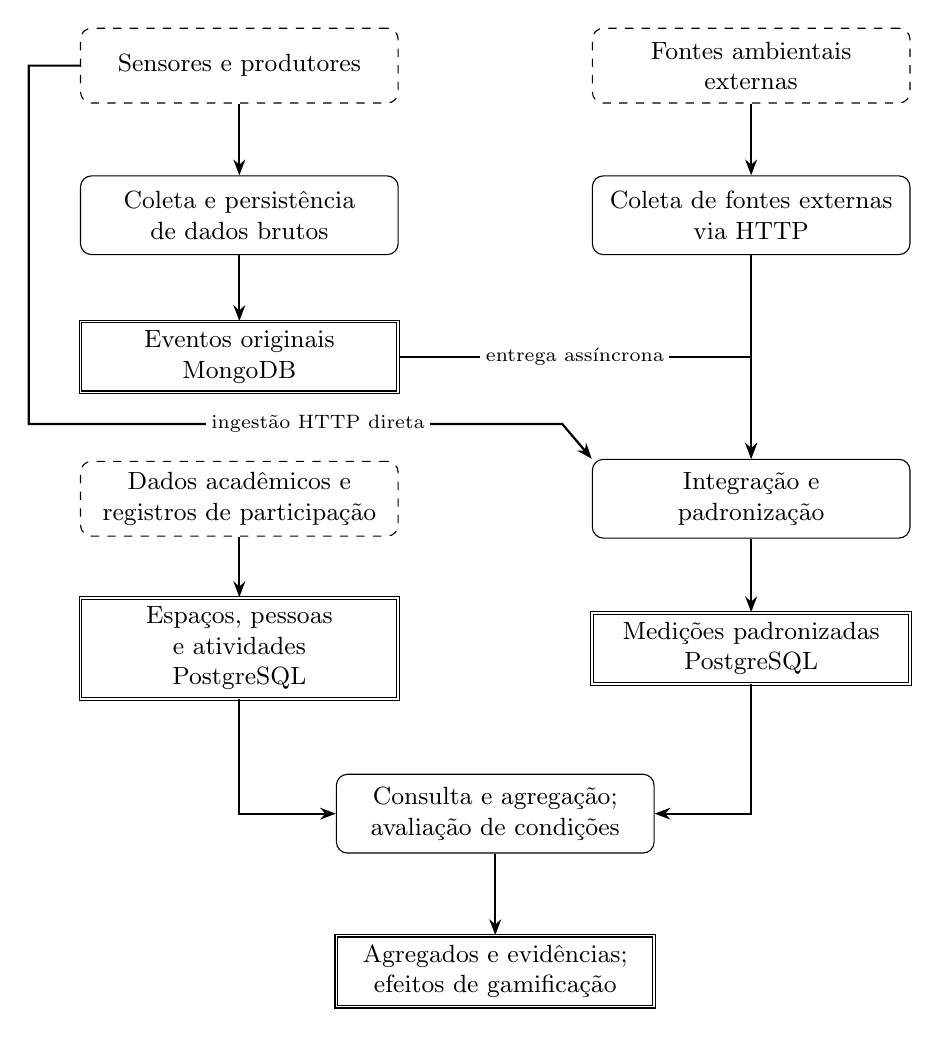
\begin{tikzpicture}[x=1cm,y=1cm,
 src/.style={draw,dashed,rounded corners,align=center,text width=3.8cm,minimum height=0.95cm,font=\small},
 proc/.style={draw,rounded corners,align=center,text width=3.8cm,minimum height=1cm,font=\small},
 dat/.style={draw,double,align=center,text width=3.8cm,minimum height=0.9cm,font=\small},
 arr/.style={-{Stealth[length=2mm]},thick},
 lab/.style={font=\scriptsize,fill=white,inner sep=2pt,align=center}]
\node[src] (s) at (0,0) {Sensores e produtores};
\node[src] (x) at (6.5,0) {Fontes ambientais\\externas};
\node[proc] (t) at (0,-1.9) {Coleta e persistência\\de dados brutos};
\node[proc] (h) at (6.5,-1.9) {Coleta de fontes externas\\via HTTP};
\node[dat] (b) at (0,-3.7) {Eventos originais\\MongoDB};
\node[proc] (i) at (6.5,-5.5) {Integração e\\padronização};
\node[dat] (c) at (6.5,-7.4) {Medições padronizadas\\PostgreSQL};
\node[src] (u) at (0,-5.5) {Dados acadêmicos e\\registros de participação};
\node[dat] (d) at (0,-7.4) {Espaços, pessoas\\e atividades\\PostgreSQL};
\node[proc] (r) at (3.25,-9.5) {Consulta e agregação;\\avaliação de condições};
\node[dat] (e) at (3.25,-11.5) {Agregados e evidências;\\efeitos de gamificação};
\draw[arr] (s)--(t); \draw[arr] (t)--(b);
\draw[arr] (x)--(h); \draw[arr] (h)--(i);
\draw[arr] (b.east)-|node[lab,pos=.25]{entrega assíncrona} (i.north);
\draw[arr] (s.west)--++(-.65,0)|-(4.1,-4.55)--(i.north west);
\node[lab] at (1,-4.55) {ingestão HTTP direta};
\draw[arr] (i)--(c); \draw[arr] (u)--(d);
\draw[arr] (c.south)|-(r.east); \draw[arr] (d.south)|-(r.west);
\draw[arr] (r)--(e);
\end{tikzpicture}
\caption*{Fonte: elaboração do autor a partir do código da versão examinada.}
\end{figure}

O serviço de coleta e persistência de dados brutos recebe mensagens por HTTP ou MQTT e preserva sua representação original no MongoDB, independentemente de já existir um perfil de integração apto a interpretar o sensor. A persistência não implica, por si só, o reconhecimento do dispositivo no domínio ou a produção de uma medição padronizada: a interpretação é uma etapa posterior. O serviço de integração, processamento e disponibilização de dados transforma entradas compatíveis com os perfis configurados e mantém no PostgreSQL as medições padronizadas e as relações acadêmicas, analíticas e de gamificação. A interface de administração e configuração permite que usuários autorizados gerenciem e consultem esses recursos. Essas responsabilidades se articulam para sustentar aplicações de gamificação sem acoplar os produtores de dados ao modelo de domínio \cite{probenAtual2026}.

O desafio arquitetural é atribuir uma responsabilidade clara a cada representação. O documento original serve à inspeção e à reinterpretação temporária; a representação comum serve a consultas e relações de domínio. A separação admite evolução independente, mas exige coordenação: não há uma transação única que inclua MongoDB e PostgreSQL. Por isso, identidade, repetição e referências entre as etapas fazem parte da solução, e não apenas detalhes de transporte.

\section{Identificar a origem: sensores, espaços e pessoas}
\subsection{Modelagem de dispositivos e grandezas}
O primeiro desafio é representar modelos de sensores sem construir uma tabela diferente para cada fabricante. A solução separa o tipo de sensor, os parâmetros que ele pode informar, o dispositivo concreto e as medições produzidas. Uma medição reúne valores numéricos, booleanos ou textuais associados a definições de parâmetro. Assim, temperatura, presença e estado de um equipamento mantêm tipos próprios, embora possam participar do mesmo fluxo de integração \cite{probenAtual2026}.

O identificador externo permite relacionar o dispositivo ao produtor que o conhece. O tipo descreve as grandezas esperadas; a configuração da integração estabelece onde encontrá-las na mensagem. Substituir um modelo exige verificar esses vínculos e sua semântica, e não apenas cadastrar um nome novo. A flexibilidade do esquema não resolve, sozinha, incompatibilidades de unidade ou calibração.

Considere, como exemplo hipotético, dois sensores de temperatura: um envia o campo \texttt{temp} e outro envia \texttt{ambient.temperature}. Se ambos expressarem graus Celsius, mapeamentos distintos podem conduzir ao mesmo parâmetro do domínio. Se uma das fontes informar outra unidade, será necessária uma transformação explicitamente suportada e validada; mudar o nome do campo não constitui conversão física. O exemplo acompanhará as etapas seguintes, sem representar uma medição de campo realizada no Centro de Artes.

\subsection{Contexto institucional e participação}
Uma observação também precisa de referência espacial. A estrutura institucional relaciona campus, prédio, unidade e compartimento, enquanto horários de aula e vínculos de estudantes permitem resolver o uso acadêmico de uma sala em determinado instante. O sistema consulta esse contexto por data e intervalo de horário e rejeita ambiguidades, em vez de escolher silenciosamente uma aula entre sobreposições \cite{probenAtual2026}.

O problema aqui é distinguir vínculo previsto de presença efetiva. Um estudante matriculado na turma pode ser elegível a uma atividade, mas isso não comprova que esteja fisicamente na sala. A versão atual mantém políticas diferentes para alunos vinculados ao uso agendado e para presença confirmada por registro de entrada e saída. Essa distinção permite que a política de beneficiários seja uma decisão explícita do domínio.

Os dados de participação não são convertidos artificialmente em leituras de sensor. Eles permanecem relacionados a pessoas, presenças, missões e atividades. A integração ocorre na interpretação: uma condição ambiental e um registro humano podem contribuir para a mesma decisão, mantendo origens identificáveis. A infraestrutura implementada dá suporte a essa relação, enquanto a experiência de interação da futura aplicação móvel permanece uma etapa separada.

\section{Receber mensagens e preservar sua identidade}
\subsection{Três caminhos de entrada}
O sistema oferece um caminho de telemetria bruta por HTTP ou MQTT, um caminho HTTP direto para medições ou formatos configurados e um coletor HTTP para fontes externas. No primeiro, o conteúdo original é registrado no MongoDB antes da entrega ao domínio. Nos demais, a integração ocorre na API e produz medições no PostgreSQL; não se deve afirmar que todas as entradas são arquivadas no MongoDB \cite{probenAtual2026}.

O caminho bruto atende ao desafio de aceitar estruturas externas antes mesmo de haver configuração para interpretá-las: a mensagem pode ser persistida com sua identidade e metadados, enquanto a produção da medição canônica depende de uma integração posteriormente configurada e válida. O caminho direto atende produtores já integrados à representação comum ou a um perfil conhecido. O coletor atende situações em que a iniciativa de consultar a fonte é do próprio sistema. A coexistência decorre dessas diferenças de interação, não de uma hierarquia em que um protocolo substitua os demais.

\subsection{Repetição, conflito e retenção}
Na telemetria bruta, a identidade combina produtor, origem e identificador de mensagem. A gravação conserva conteúdo, instantes e estado de processamento. Uma retransmissão equivalente é reconhecida; conteúdo divergente sob a mesma identidade gera conflito. No MQTT, o produtor é obtido do tópico, e a identificação da mensagem da aplicação não é substituída pelo identificador de pacote do protocolo \cite{probenAtual2026,oasisMqtt2019}.

O desafio de confiabilidade é que uma confirmação de transporte encerra apenas uma etapa. O recebimento MQTT usa confirmação manual após persistência ou decisão permanente; falha transitória de armazenamento permite reentrega. Isso não significa que a interpretação, a missão ou a recompensa tenham terminado. A identidade precisa atravessar as etapas para que a repetição necessária à recuperação não multiplique efeitos de domínio.

A preservação é temporária. \emph{Time to Live} (TTL) é o prazo de retenção utilizado para expirar os documentos brutos; a configuração geral documentada é de 30 dias. Depois desse período, a medição e seus metadados podem permanecer no modelo relacional, mas o conteúdo original deixa de estar disponível para nova interpretação. Auditoria permanente do conteúdo bruto exigiria outra política de armazenamento.

\section{Transformar a mensagem em uma medição comum}
\subsection{Integração configurável e versões de interpretação}
O próximo desafio é impedir que o formato de cada dispositivo se propague pelas consultas e regras. Perfis de integração descrevem seleção de sensor, campos de tempo e valores e vínculos com dispositivos. O \emph{parser}, componente que interpreta a estrutura recebida, utiliza uma versão identificada; mapeamentos por JSON Pointer permitem apontar campos do documento \cite{jsonpointer2013,probenAtual2026}.

No exemplo, os campos \texttt{temp} e \texttt{ambient.temperature} são interpretados por configurações diferentes, mas a leitura resultante passa a ser um valor numérico de um parâmetro definido. O domínio não precisa conhecer o nome externo do campo para consultar a temperatura. Essa separação é a contribuição prática da representação comum: estabilizar a relação entre grandeza, sensor e instante.

Versões e vínculos também precisam continuar válidos no momento da gravação. O código atual revalida o perfil, a versão ativa e o vínculo do dispositivo dentro da operação de ingestão. Esse cuidado procura tratar a alteração concorrente de uma configuração entre sua consulta e seu uso. A versão utilizada fica associada aos metadados da ingestão, apoiando a explicação posterior do resultado.

\subsection{Idempotência na fronteira relacional}
A medição e os metadados são persistidos em uma transação local. O orquestrador distingue ingestão direta, por perfil e originada na telemetria, com restrições próprias para as respectivas identidades. A comparação de uma impressão do conteúdo, ou \emph{fingerprint}, permite distinguir repetição equivalente de conflito \cite{probenAtual2026}.

Esse mecanismo responde a um caso concreto: a API pode concluir a gravação e a resposta não chegar ao serviço de coleta e persistência de dados brutos. Repetir a entrega é necessário, mas criar uma nova medição seria incorreto. A solução combina identidade persistida e leitura do resultado já existente. O desenho trata essa fronteira por repetição segura; sua comprovação sob interrupção real exatamente entre os dois bancos permanece um cenário experimental específico.

\subsection{Retomada e reinterpretação}
O processamento assíncrono registra trabalho pendente, reservado, concluído ou falho. Reservas temporárias permitem recuperar itens interrompidos; tentativas e espera crescente reduzem a repetição imediata de falhas transitórias. No reprocessamento administrativo, o conteúdo original e a identidade são preservados, com registro do pedido e do estado anterior \cite{probenAtual2026}.

Reprocessar não é necessariamente reproduzir a interpretação original: a seleção pode usar a configuração ativa no novo processamento. Essa diferença deve ser visível ao operador e ao leitor. O resultado pode ser equivalente, conflitante ou falho, mas não deve sobrescrever silenciosamente uma medição anterior. A flexibilidade obtida pela preservação documental exige, em contrapartida, governança das versões e das decisões de reinterpretação.

\section{Acrescentar contexto externo sem replicar observações}
\subsection{Fontes compartilhadas e localização}
A temperatura externa não pertence exclusivamente a uma sala. Replicá-la como leitura independente de cada compartimento criaria dados redundantes e obscureceria sua origem. A solução atual representa um contexto compartilhado, com vínculos explícitos às salas e uma seleção de fonte por compartimento e parâmetro. O sensor pertence a um compartimento ou a um contexto compartilhado, sem criar salas fictícias para acomodar uma fonte externa \cite{probenAtual2026}.

O coletor consulta um serviço externo por HTTP, interpreta a resposta e utiliza o mesmo núcleo de ingestão das medições. Método, parâmetros, cabeçalhos, mapeamentos e interpretação do tempo são configuráveis. As credenciais administradas são armazenadas de forma cifrada, e a interface oferece teste de configuração. A flexibilidade do coletor amplia as possibilidades de integração, mas cada serviço ainda exige configuração e validação de seu contrato.

A localização é parte da identidade da observação. As coordenadas podem pertencer ao próprio contexto ou ser obtidas do campus. O registro de coleta associa a medição à localização utilizada e a uma impressão geográfica. Consultas atuais rejeitam observações de uma localização antiga quando as coordenadas mudam. Isso evita que uma série aparentemente contínua combine dados referentes a lugares diferentes.

Uma nova observação compartilhada é um fato disponível às próximas avaliações; ela não é multiplicada em novas medições por sala. Na ingestão atual, somente sensores locais criam diretamente a solicitação de avaliação de missão. A distinção entre disponibilizar contexto e disparar uma avaliação evita interpretar um dado meteorológico como ação independente de cada sala.

\subsection{Validade e cobertura temporal}
Uma ausência de resposta não representa temperatura zero. A consulta de uma fonte compartilhada distingue informação disponível, desatualizada e ausente. Regras que dependem de dados sem validade suficiente recebem um motivo de não avaliação. Esse tratamento protege a interpretação: atribuir um valor numérico à ausência alteraria médias e decisões sem que houvesse uma observação correspondente.

Para a referência externa de sete dias, a implementação calcula uma média por tempo coberto. Considerando observações ordenadas $(t_i,v_i)$ dentro da janela, a política utiliza:
\begin{equation}\label{eq:media-externa}
\overline{T}_{e,7d}=\frac{\sum_i v_i\Delta_i}{\sum_i\Delta_i},\qquad
\Delta_i=\min(t_{i+1}-t_i,3600\,\mathrm{s}).
\end{equation}
Instantes repetidos são consolidados; cada observação contribui até a próxima, limitada a uma hora. O cálculo requer pelo menos 120 horas cobertas nas 168 horas da janela. Não há extensão implícita do último ponto até o fim. Essa é uma política de disponibilidade e agregação implementada no projeto, não uma prescrição geral da literatura de conforto \cite{probenAtual2026}.

O limite de uma hora procura impedir que uma única leitura cubra uma interrupção longa. O mínimo de cobertura evita apresentar uma média de poucos pontos como representativa de sete dias. Essas escolhas têm custos: uma sequência com lacunas pode impedir a avaliação mesmo contendo algumas leituras recentes. Sua adequação às condições reais do provedor e do prédio deverá ser examinada na operação.

\section{Consultar e resumir as medições}
Uma vez padronizadas, as medições podem ser consultadas ou agrupadas por período. O desafio é definir o que cada resumo representa e permitir retomar seu cálculo. A agregação é organizada em janelas persistidas, com início incluído e fim excluído, representadas por $[t_i,t_f)$. Essa convenção impede que uma leitura na fronteira seja incluída em duas janelas adjacentes \cite{akidau2015,probenAtual2026}.

Os agregados numéricos armazenam média, mínimo, máximo e quantidade de amostras. A média de uma janela é aritmética por amostra. Ao combinar agregados, a média é ponderada por essa quantidade, e não pela duração de cada leitura. Trata-se de uma política diferente da Equação~\ref{eq:media-externa}; confundi-las levaria a conclusões incorretas sobre sensores com frequências distintas.

As janelas de agregação também usam estados, reserva temporária e repetição. Uma medição atrasada pode exigir recomputação explícita de um resultado já encerrado. O sistema não é apresentado como um mecanismo completo de processamento contínuo que atualiza automaticamente todos os agregados diante de qualquer atraso. O console disponibiliza filtros e visualização de agregados, mas sua existência não substitui a análise da semântica do cálculo.

\section{Interpretar condições e relacioná-las às atividades}
\subsection{Qualificação de valores e eventos de missão}
O dado padronizado permite expressar condições sem depender do formato do fabricante. Uma regra de qualificação pode comparar uma temperatura a limites e registrar o resultado associado ao valor. Uma condição de evento de missão pode utilizar o valor diretamente ou uma avaliação de regra. Assim, a interpretação pode ser reutilizada, desde que a política aplicável permaneça identificável \cite{probenAtual2026}.

As avaliações elementares não precisam ser mutuamente exclusivas. Uma temperatura pode satisfazer simultaneamente um limiar de alerta e outro mais severo. A versão inspecionada não deve ser descrita como escolhendo automaticamente um único resultado apenas pela existência de uma coluna de prioridade. Consolidar resultados exige uma política explícita, diferente de registrar cada regra satisfeita.

Missões relacionam condições, ocorrências, atividades e beneficiários. Algumas condições são instantâneas; outras dependem de duração, transição ou encerramento de uma janela. Nesses casos, tempo e lacunas fazem parte da interpretação. Estados e evidências persistidos permitem explicar o progresso e retomar uma janela, sem reduzir uma condição temporal à comparação da última leitura.

O motor simples permanece a opção padrão para as regras instantâneas. Drools é uma alternativa experimental para avaliação temporal, habilitada por configuração. A lógica de comparação fica separada dos efeitos persistentes, evitando que a avaliação de uma regra execute diretamente operações de recompensa. O experimento histórico que motivou essa escolha é analisado no Capítulo~\ref{cap:avaliacao}.

\subsection{Regras de ambiente e precedência de escopo}
A versão atual acrescenta um fluxo próprio de regras de ambiente. Ele reutiliza medições locais, fontes compartilhadas, contexto acadêmico e registro de pontos, mas não exige transformar cada verificação agendada em uma missão ou atividade. As categorias iniciais incluem ar-condicionado, iluminação e equipamentos; a configuração aceita operadores declarativos, sem código arbitrário fornecido pelo usuário \cite{probenAtual2026}.

O desafio de replicação institucional aparece na escolha da regra efetiva. Para cada sala e categoria, uma regra específica tem precedência; na ausência dela, aplica-se o padrão do campus e, depois, o padrão global. A regra de menor abrangência substitui o padrão nesse contexto, evitando executá-los como se fossem verificações independentes equivalentes. Ambiguidades e conflitos de escopo são tratados explicitamente.

Cada execução registra uma cópia da configuração utilizada, ou \emph{snapshot}, além do instante previsto e das evidências. Alterar a regra posteriormente não altera essa cópia. A conclusão da execução e a concessão de pontos verificam a posse válida da reserva temporária. Essa organização procura impedir que um executor antigo, após perder a reserva, conclua o trabalho que já foi retomado por outro.

\subsection{Faixa adaptativa: dados, cálculo e limites}\label{sec:conforto}
A configuração de conforto adaptativo combina uma temperatura interna com a referência externa de sete dias. O componente atual calcula a temperatura neutra $T_n$ e os limites $L$ e $U$ por:
\begin{align}
T_n &=17{,}8+0{,}31\overline{T}_{e,7d},\\
L &=T_n-d_{\mathrm{inf}},\qquad U=T_n+d_{\mathrm{sup}}.
\end{align}
As diferenças inferior e superior são configuráveis e assumem $3{,}5\,^{\circ}\mathrm{C}$ como valor padrão. A comparação implementada inclui os dois limites. Esses valores descrevem o código examinado; o fundamento adaptativo remete à relação entre experiência térmica externa e condições internas discutida por De Dear e Brager \cite{deDear2002,probenAtual2026}.

Se a média externa for $20\,^{\circ}\mathrm{C}$, o cálculo produz $T_n=24\,^{\circ}\mathrm{C}$ e, com os afastamentos configurados por padrão, a faixa de $20{,}5$ a $27{,}5\,^{\circ}\mathrm{C}$. A temperatura interna de $22{,}5\,^{\circ}\mathrm{C}$ do exemplo está nessa faixa. Isso descreve uma condição aritmética; não comprova conforto de um ocupante, nem economia de energia.

A aplicação científica do modelo exige cautela. O estudo de referência trata ambientes naturalmente ventilados e utiliza temperatura operativa em sua avaliação. O software opera com os parâmetros fornecidos pela integração e uma política própria de média externa. Não há verificação automática de todas as condições ambientais e de ocupação exigidas para uma aplicação normativa. A variável interna configurada também não é automaticamente equivalente à temperatura operativa. Assim, a infraestrutura torna o cálculo disponível e rastreável, mas sua utilização em uma intervenção requer validação de domínio.

Condições adicionais, como estado de um equipamento e ocupação, continuam necessárias quando configuradas. A faixa adaptativa não as substitui. Dados ausentes, antigos ou com cobertura insuficiente impedem o uso da condição correspondente; a execução registra o motivo, em vez de preencher lacunas com zero ou conceder pontos a partir de uma informação inexistente.

\section{Dos resultados aos efeitos de gamificação}
O último desafio do percurso é relacionar uma decisão a pessoas sem perder sua evidência nem repetir seu efeito. Em missões, ocorrências podem progredir atividades e gerar pontos. Em regras de ambiente, a execução identifica contexto, beneficiários e resultado antes de registrar o efeito. O saldo de \emph{Experience Points} (XP), pontos de experiência, é calculado pela soma de lançamentos em um \emph{ledger}, registro de movimentações preservadas, em vez de substituir continuamente um saldo na pessoa \cite{probenAtual2026}.

\begin{figure}[htbp]\centering
\caption{Relações conceituais necessárias para explicar um efeito de gamificação. A implementação concreta difere entre missões e regras de ambiente.}
\label{fig:rastreabilidade}
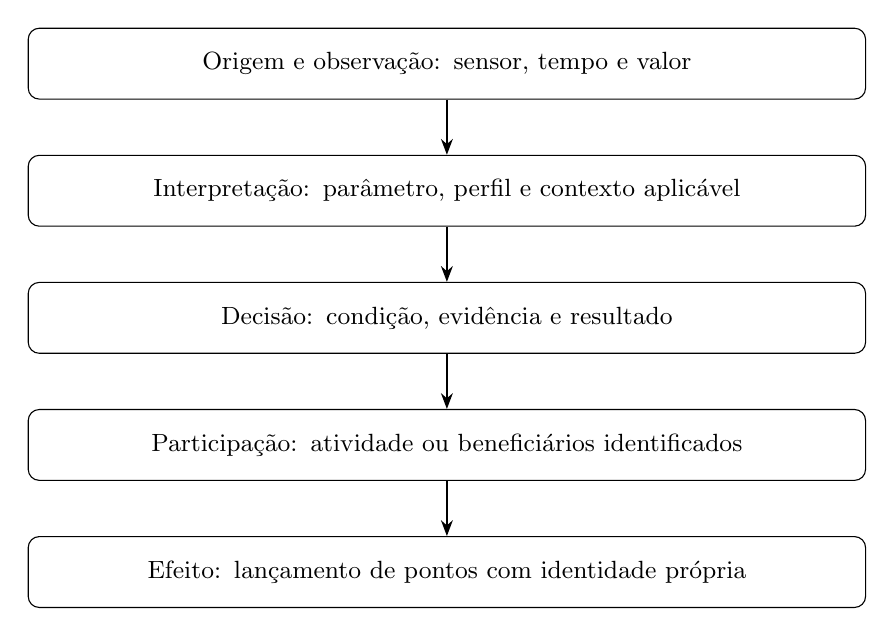
\begin{tikzpicture}[node distance=7mm,
 box/.style={draw,rounded corners,align=center,text width=10.4cm,minimum height=9mm,font=\small},
 arr/.style={-{Stealth[length=2mm]},thick}]
\node[box] (a) {Origem e observação: sensor, tempo e valor};
\node[box,below=of a] (b) {Interpretação: parâmetro, perfil e contexto aplicável};
\node[box,below=of b] (c) {Decisão: condição, evidência e resultado};
\node[box,below=of c] (d) {Participação: atividade ou beneficiários identificados};
\node[box,below=of d] (e) {Efeito: lançamento de pontos com identidade própria};
\draw[arr] (a)--(b);\draw[arr] (b)--(c);\draw[arr] (c)--(d);\draw[arr] (d)--(e);
\end{tikzpicture}
\caption*{Fonte: elaboração do autor a partir do código da versão examinada.}
\end{figure}

A Figura~\ref{fig:rastreabilidade} sintetiza o argumento: um ponto deve estar relacionado à decisão que o produziu, e a decisão aos dados que a sustentaram. Na telemetria, identificadores relacionam documento bruto e medição; no domínio relacional, referências conectam valores, evidências, ocorrências e atividades. As regras de ambiente acrescentam cópia da configuração de execução e referências aos seus lançamentos.

Essa rastreabilidade tem limites diferentes. O conteúdo bruto desaparece após a retenção; a ligação entre bancos é lógica, não uma chave estrangeira distribuída; e regras elementares de qualificação não necessariamente preservam todos os limiares históricos dentro de cada avaliação. O \emph{snapshot} das regras de ambiente melhora a explicação nesse fluxo, mas não autoriza afirmar que todas as políticas históricas de todo o sistema são integralmente reconstruíveis.

\section{Operação e proteção ao longo do percurso}
O console permite configurar sensores, integrações, fontes compartilhadas, missões e regras, além de consultar medições e agregados. Esse suporte operacional é relevante porque a adaptação de fontes precisa ser realizável sem alterar o código a cada configuração. As capturas do Apêndice~\ref{ap:console} ilustram funcionalidades já documentadas; por serem anteriores à atualização, não são apresentadas como prova visual de todas as telas atuais.

A identidade e os papéis controlam quais operações cada cliente pode executar. \emph{JSON Web Token} (JWT) é o formato de token empregado para transportar informações da autenticação \cite{jwt2015}. Há separação entre usuários humanos, produtores de ingestão e a identidade técnica de comunicação entre serviços. O \emph{Role-Based Access Control}, controle por papéis, organiza responsabilidades administrativas, operacionais, analíticas e de participação. Seu emprego responde à necessidade de impedir que receber dados implique também poder alterar usuários ou configurações sensíveis.

Estados, métricas e registros de execução tornam o processamento observável. O problema é localizar uma falha sem depender de um resultado final ausente. Por isso, identificar se um item foi recebido, interpretado, rejeitado ou retomado faz parte do percurso. As políticas de proteção e observação também têm limites de implantação: a autenticidade do produtor MQTT depende da configuração do intermediário, e a existência de autenticação na aplicação não substitui uma auditoria completa de segurança \cite{probenAtual2026}.

\chapter{Avaliação e Discussão}\label{cap:avaliacao}
A avaliação retoma os desafios do percurso para examinar o que o artefato permite demonstrar. São separados três níveis de evidência: mecanismos e cenários identificados no código atual, registros históricos de execução e resultados de um experimento anterior. A separação evita que uma ampliação funcional seja interpretada como aprovação automática de toda a versão.

\section{Inspeção da versão atual}
A Tabela~\ref{tab:avaliacao} relaciona requisitos, mecanismos e cenários localizados no commit definido na Seção~\ref{sec:versoes}. ``Cenário localizado'' significa leitura do código de teste e de seu oráculo; não uma nova execução aprovada. As classes são identificadas no Apêndice~\ref{ap:evidencias}, mantendo os nomes de implementação fora do argumento principal.

\begin{table}[htbp]\centering\small
\caption{Mecanismos e cenários identificados na versão atual}\label{tab:avaliacao}
\begin{tabularx}{\textwidth}{p{1.2cm}p{2.9cm}YY}\toprule
Req. & Propriedade & Mecanismo ou cenário localizado & Alcance da evidência \\\midrule
R1--R4 & Integração e identidade & Recebimento bruto, ingestão direta e por perfil, comparação de conteúdo e validação transacional. & Estrutura inspecionada; diversidade real de fabricantes não demonstrada. \\
R5 & Fonte compartilhada & Seleção explícita, mesma observação usada por várias salas, rejeição de localização antiga e cobertura insuficiente. & Código de serviço e de testes; execução atual não aferida. \\
R6 & Agregação temporal & Persistência de janelas e agregados; distinção entre média por amostra e média externa ponderada no tempo. & Semântica descrita; carga e atraso contínuo não medidos. \\
R7--R8 & Efeitos e recuperação & Reserva recuperável, posse da execução e identidade de lançamento por beneficiário. & Cenários de concorrência e perda de reserva localizados, sem ensaio distribuído completo. \\
R9 & Operação e proteção & Separação de serviços e identidades; cenários de proteção do coletor. & Não equivale a auditoria de segurança ou usabilidade. \\
R10 & Regras de ambiente & Precedência de escopo, contexto, presença, cópia de configuração e limites adaptativos. & Consistência do desenho examinada; efeito em campo não avaliado. \\\bottomrule
\end{tabularx}
\caption*{Fonte: inspeção do código e dos testes no commit de referência \cite{probenAtual2026}.}
\end{table}

Os testes atuais de conforto incluem comparações nos limites da faixa e condições imediatamente externas, exigência de fatos adicionais e ausência de informação. Os de fontes compartilhadas distinguem validade, localização, reutilização da observação e cobertura da média. Os de regras de ambiente incluem precedência entre sala, campus e padrão global, preservação da configuração e recuperação de reserva. Esses oráculos correspondem aos riscos discutidos no desenvolvimento, mas precisam ser executados e arquivados no mesmo commit para produzir um resultado consolidado \cite{probenAtual2026}.

Há uma diferença entre impedir repetição por restrição local e demonstrar consistência de ponta a ponta. O caso em que a API conclui e o serviço de coleta de dados brutos perde a confirmação é tratado pelo desenho de ingestão, mas permanece necessária uma execução controlada com interrupção nessa fronteira. Da mesma forma, uma simulação de perda de reserva não equivale a uma indisponibilidade longa envolvendo processos, rede e bancos.

\section{Registros históricos de verificação}
O relatório de testes de sanidade de 17 de setembro de 2026 registra 112 verificações aprovadas, cinco avisos e zero falhas em 71,6 segundos, contra um ambiente identificado como produção. Entre os avisos estavam timeout na sincronização de salas, falha de autenticação ao consultar um processamento de horários e a verificação de persistência não realizada em consequência, além de estados tolerados de usuário já existente e presença já encerrada \cite{probenSmoke2026}.

O relatório é uma evidência operacional daquele roteiro e instante. Ele não identifica o hash implantado e antecede a versão atual; por isso, não valida as novas fontes externas ou as regras de ambiente. O tempo total mistura rede, espera e operações distintas e não é tratado como medida de desempenho da arquitetura.

\section{Experimento histórico dos motores de regras}
O documento de decisão sobre Drools registra um experimento com \emph{Java Microbenchmark Harness}, ferramenta para medição de operações Java em condições controladas. A configuração utilizou dois processos de execução independentes, cinco iterações de aquecimento e dez de medição, de um segundo cada, com OpenJDK 21.0.10 em Windows 11. O próprio documento informa que o hardware não foi identificado automaticamente. O registro não vincula de modo suficiente todos os resultados a um hash executado e a um ambiente dedicado; esses limites são preservados nesta análise \cite{probenDrools2026}.

O experimento compara um motor simples com Drools em dois estados. Na operação fria, a criação e compilação da base de regras são incluídas. Na operação quente, a base compilada é reutilizada, mas uma sessão é criada para cada avaliação. Cada operação avalia um lote completo de fatos, sem rede, persistência e demais executores da aplicação. A Tabela~\ref{tab:benchmark} reproduz apenas os resultados do cenário instantâneo com mil fatos, para o qual existe comparação entre as três configurações.

\begin{table}[htbp]\centering\small
\caption{Resultados históricos para um lote de mil fatos instantâneos}\label{tab:benchmark}
\begin{tabularx}{\textwidth}{Yrr}\toprule
Configuração & Latência média (ms) & Percentil 99 (ms) \\\midrule
Motor simples & 0,016 & 0,049 \\
Drools com compilação por operação & 44,619 & 97,750 \\
Drools com base reutilizada & 1,502 & 3,011 \\\bottomrule
\end{tabularx}
\caption*{Fonte: documento de decisão técnica do projeto \cite{probenDrools2026}.}
\end{table}

O percentil 99 é o valor abaixo do qual se encontram aproximadamente 99\% das amostras de latência do cenário. Os números apoiam a escolha do motor simples para as regras instantâneas medidas. Não demonstram que ele seja superior em toda regra temporal nem representam tempo de resposta de uma missão completa. O documento também relata Drools em cenários de duração, mas sem resultado equivalente do motor simples; essa parte não sustenta uma comparação de superioridade.

O resultado é relevante como justificativa de uma decisão anterior, não como medição da versão atual. Para reavaliar a escolha, é necessário fixar código e ambiente, repetir o experimento e incluir regras representativas do uso esperado. O cálculo de regras de ambiente, por sua vez, é um fluxo próprio e não deve receber os números desse experimento como se medisse o mesmo mecanismo.

\section{Discussão por desafio de projeto}
\subsection{Flexibilidade de integração e custo de coordenação}
A separação entre mensagem original e representação comum permite interpretar formatos sem alterar cada consumidor. Perfis e parâmetros tornam essa flexibilidade operável. Entretanto, a necessidade de dois armazenamentos acrescenta fronteiras de falha, referências lógicas e políticas de retenção. A contribuição do desenho é explicitar e tratar essas fronteiras; a avaliação disponível não prova vantagem de desempenho em relação a uma arquitetura com banco único.

\subsection{Contexto e qualidade da decisão}
Os dados compartilhados reduzem replicação e preservam origem, enquanto validade e cobertura impedem preencher lacunas como se fossem observações. Em contrapartida, uma decisão pode deixar de ser executada por falta de dados, e a alteração de localização pode exigir reconstruir o histórico disponível. Esses resultados não são defeitos necessariamente: tornam explícita a dependência entre qualidade da entrada e possibilidade de interpretação.

A relação entre matrícula, horário e presença também impede equiparar automaticamente participantes previstos e presentes. O sistema oferece políticas distintas, mas o projeto institucional ainda precisa decidir qual delas é adequada para cada atividade. A infraestrutura torna a escolha representável e auditável; sua legitimidade pedagógica e comportamental depende da intervenção.

\subsection{Rastreabilidade e limites de comprovação}
Identidades, referências e cópias de configuração permitem inspecionar por que um resultado foi produzido. Isso sustenta a explicabilidade técnica de partes do percurso. A preservação temporária do bruto e as diferenças de versionamento entre tipos de regra limitam a reconstrução completa. É necessário avaliar explicitamente o que deve ser retido, por quanto tempo e em qual nível de detalhe antes de afirmar auditoria integral.

\section{Ameaças à validade e avaliação ainda necessária}
A validade interna é limitada pela autoria comum do sistema e de seus testes, pela ausência de nova execução consolidada na versão atual e pela falta de um ensaio completo de falha entre os bancos. A inspeção confirma mecanismos e intenções de teste, mas não todos os comportamentos em execução.

A validade externa é limitada ao contexto institucional e aos formatos examinados no desenvolvimento. Não foi demonstrada carga representativa de um prédio ocupado nem operação prolongada em múltiplas unidades. Modularidade e configurações favorecem a intenção de expansão, mas não constituem medição de escalabilidade.

A validade de construto exige distinguir condição calculada, conforto, engajamento e economia. Pontos não medem consumo evitado, uma matrícula não comprova presença e uma faixa térmica implementada não comprova conforto percebido. O estudo de campo deverá definir linha de base, métricas, critérios de aplicação do modelo e instrumentos apropriados aos objetivos institucionais.

Para fortalecer a avaliação técnica, são necessários um pacote de execução vinculado ao commit atual, testes de interrupção entre serviços, comparação de formatos equivalentes, carga contínua e ensaios de restauração. A avaliação de segurança e usabilidade exige procedimentos próprios. Essas lacunas delimitam o que se pode concluir a partir do artefato apresentado.

\chapter{Conclusão}\label{cap:conclusao}
Este trabalho investigou a construção de uma infraestrutura capaz de relacionar observações ambientais heterogêneas e registros de participação para apoiar a gamificação da eficiência energética. O cenário do Centro de Artes da UFPel permitiu formular o problema como um percurso de integração: identificar a origem, receber dados, preservar evidências, produzir uma representação comum, acrescentar contexto e utilizar as informações em análises e decisões.

A solução implementada combina preservação documental temporária e persistência relacional, perfis configuráveis de integração, fontes externas compartilhadas e relações acadêmicas e de participação. Agregação, missões e regras de ambiente utilizam essa base com mecanismos de identidade, estados e recuperação. A versão atual também registra configurações e evidências de execução de regras de ambiente, incluindo o cálculo de uma faixa adaptativa a partir de dados internos e externos.

Em resposta à questão de pesquisa, o artefato mostra uma forma concreta de separar a variabilidade das fontes das relações estáveis necessárias ao domínio, mantendo vínculos entre observações e efeitos. A principal contribuição não está em uma tecnologia isolada, mas na articulação desses mecanismos e na explicitação dos desafios de integração, tempo, contexto e repetição.

A avaliação disponível sustenta conclusões delimitadas. A inspeção atual identifica mecanismos e cenários; o relatório operacional e o experimento de motores constituem evidências históricas. Eles não substituem uma execução consolidada da versão atual nem demonstram economia, conforto em campo ou escalabilidade institucional. O motor simples permanece justificado nos cenários instantâneos historicamente medidos, sem transferir esse resultado para todos os fluxos.

A continuidade do trabalho deve priorizar a consolidação das evidências técnicas, o versionamento das políticas históricas e os ensaios de carga e recuperação. Em paralelo, a integração da aplicação móvel permitirá avaliar a participação no uso real. A validação do conforto e do impacto energético deverá ocorrer no projeto institucional, com critérios de domínio e desenho de avaliação apropriados. A infraestrutura apresentada constitui a base de dados e serviços para essa etapa.

\appendix
\chapter{Fontes Técnicas e Reprodução da Análise}\label{ap:evidencias}
Este apêndice identifica o material de implementação utilizado para fundamentar a descrição do sistema. Os caminhos são relativos ao repositório técnico e pertencem ao commit \path{5e2a1e27d2f4ceb31217867259a303eee84b3c0f}. A lista organiza a conferência do percurso; não constitui um relatório de execução das suítes.

\begin{longtable}{p{3.1cm}p{9.8cm}}
\caption{Componentes utilizados na inspeção do fluxo atual}\label{tab:fontes-codigo}\\
\toprule Etapa & Evidência de implementação \\\midrule\endfirsthead
\toprule Etapa & Evidência de implementação \\\midrule\endhead
Recebimento e entrega & \path{Proben-Telemetry/src/main/java/com/proben/telemetry/service/canonical/CanonicalTelemetryWorker.java}; \path{RawTelemetryClaimService.java} no mesmo pacote; \path{Documentos/MQTT.md}. \\
Integração & \path{Proben-API/src/main/java/com/proben/api/service/sensors/SensorIngestOrchestrator.java}; \path{SensorCanonicalIngestionTransaction.java}; \path{SensorIngestionService.java}. \\
Fontes externas & \path{Proben-API/src/main/java/com/proben/api/service/shared/SharedContextService.java}; \path{SharedContextCollector.java}; \path{CredentialEncryptionService.java}. \\
Contexto acadêmico & \path{Proben-API/src/main/java/com/proben/api/service/academic/AcademicContextResolver.java}; \path{service/missions/beneficiaries/DefaultMissionBeneficiaryResolver.java}. \\
Regras de ambiente & \path{Proben-API/src/main/java/com/proben/api/service/environment/EnvironmentRuleService.java}; \path{EnvironmentRuleWorker.java}; \path{AdaptiveComfortCalculator.java}. \\
Estrutura persistida & \path{Proben-API/src/main/resources/db/migration/}, especialmente V29 a V33 para contextos, coleta e regras de ambiente. \\
Documentação & \path{README.md}; \path{Documentos/Catalogo-Dados.md}; \path{Documentos/Modelo-MongoDB/Modelo-Telemetria-MongoDB.md}; \path{Documentos/Organizacao-do-Codigo.md}. \\\bottomrule
\end{longtable}
{\footnotesize Fonte: inspeção do repositório técnico pelo autor \cite{probenAtual2026}.\par}

No diretório de testes de regras de ambiente foram examinados cenários de resolução, histórico, concorrência, integração acadêmica, fontes compartilhadas e conforto adaptativo. Em particular, \path{EnvironmentRuleResolutionIntegrationTest} trata precedência e reserva; \path{EnvironmentRuleSharedContextIntegrationTest} trata localização e cobertura; \path{EnvironmentRuleAdaptiveComfortIntegrationTest} trata limites e fatos obrigatórios. O conjunto de fontes compartilhadas também contém cenários de falha, posse de reserva e proteção da coleta. A presença de Testcontainers com opção de ignorar testes sem Docker exige registrar separadamente casos executados e ignorados em uma futura execução.

Para reprodução da análise, deve-se obter o commit identificado e conferir os módulos \path{Proben-API}, \path{Proben-Telemetry} e \path{Proben-Admin}. Uma execução de testes pode utilizar \path{./Proben-API/mvnw -f Proben-API/pom.xml test} e \path{./Proben-API/mvnw -f Proben-Telemetry/pom.xml test}, com ambiente Java e Docker compatíveis; o console utiliza seus comandos definidos no arquivo de dependências. O benchmark é uma etapa separada, descrita em \path{Documentos/Decisao-Drools-POC.md}. Os resultados precisam registrar hash, ambiente, comando, falhas e casos ignorados.

Os documentos históricos continuam identificados pelo commit antigo nas respectivas referências. Resultados locais sem arquivo preservado não são convertidos em evidência atual. Uma versão de entrega deverá arquivar relatórios e resultados brutos junto de uma identificação permanente do código correspondente.

\chapter{Exemplos Documentados do Console}\label{ap:console}
As capturas a seguir, já presentes no material anterior do TCC, ilustram a relação entre conceitos do domínio e operação. Elas foram produzidas antes da renomeação e mostram ``PROCEL Console''. São registros históricos de interface, não capturas da versão atual nem evidência de usabilidade. As novas telas de fontes compartilhadas e regras de ambiente não são inferidas a partir delas.

\begin{figure}[htbp]\centering
\caption{Registro histórico do console: medições e qualificação.}
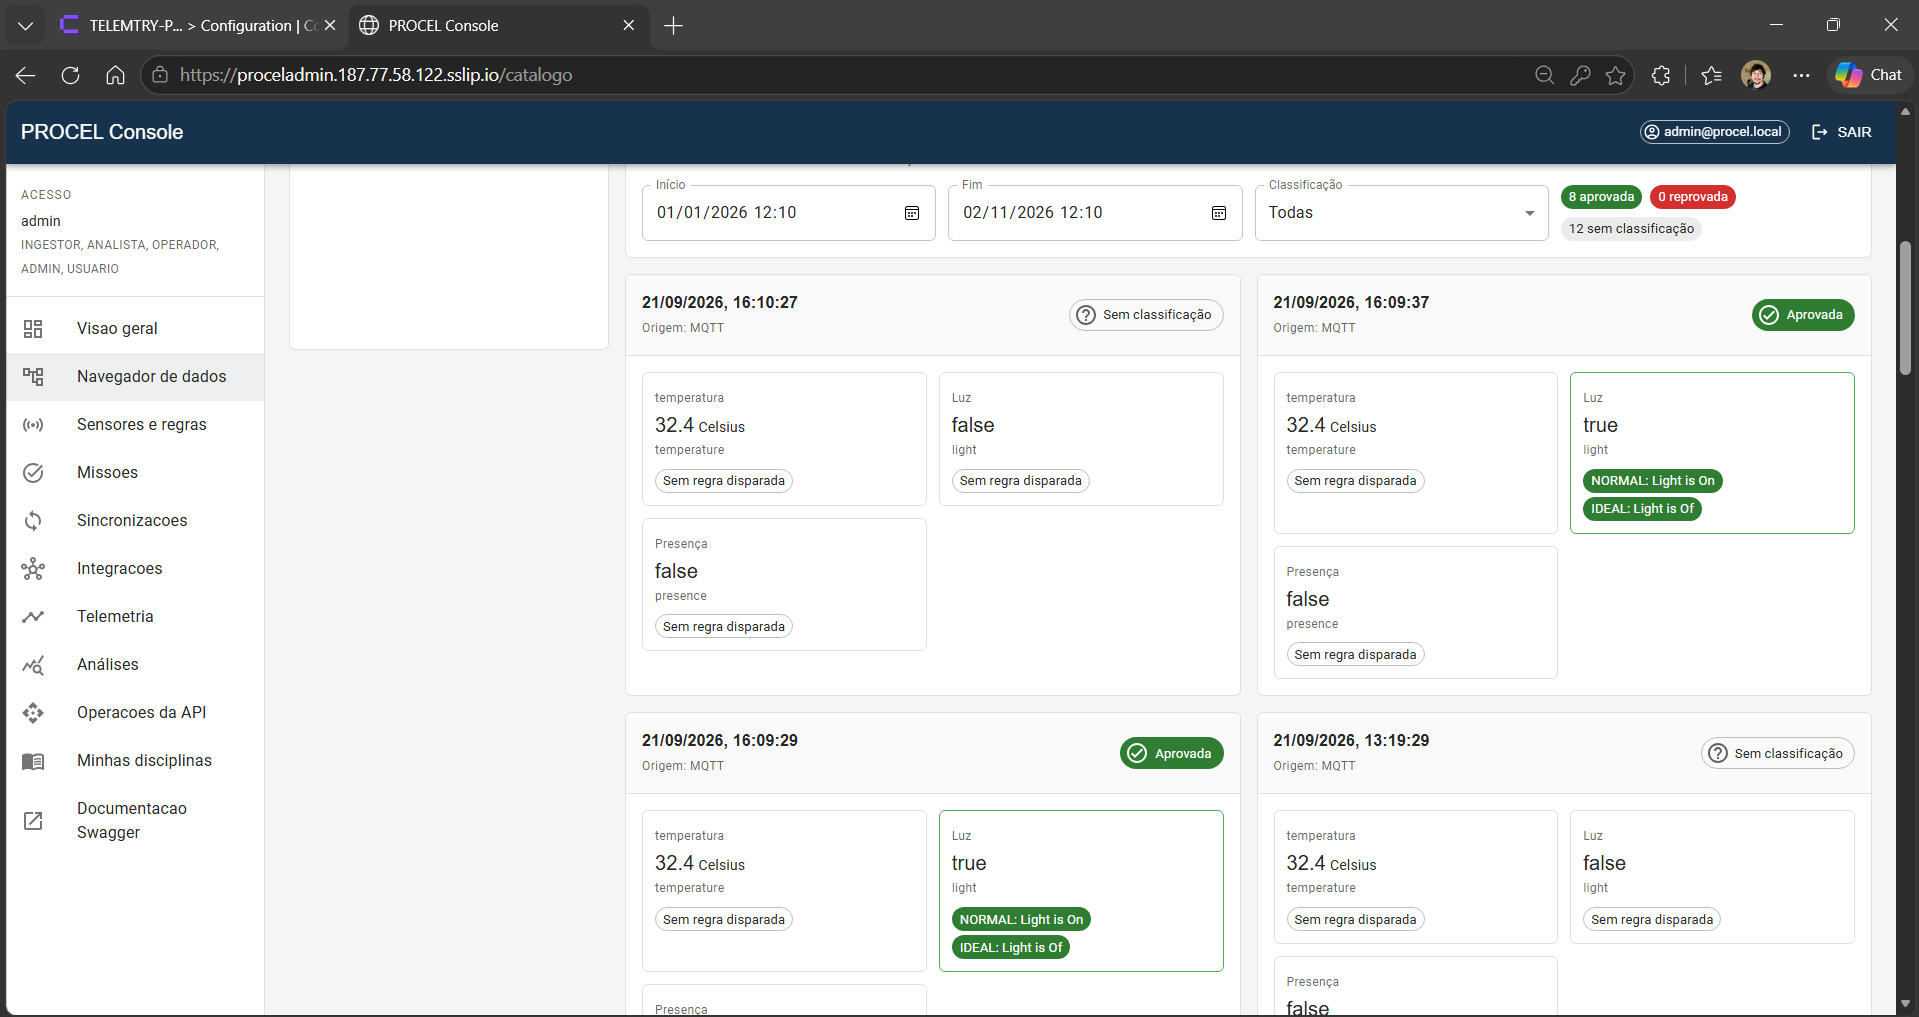
\includegraphics[width=\textwidth,trim=0 0 0 75,clip]{imagens/screenshots-do-PROCEL/Screenshot_2.png}
\caption*{Fonte: captura histórica do console fornecida pelo autor.}
\end{figure}
\begin{figure}[htbp]\centering
\caption{Registro histórico do console: grupos e regras de qualificação.}
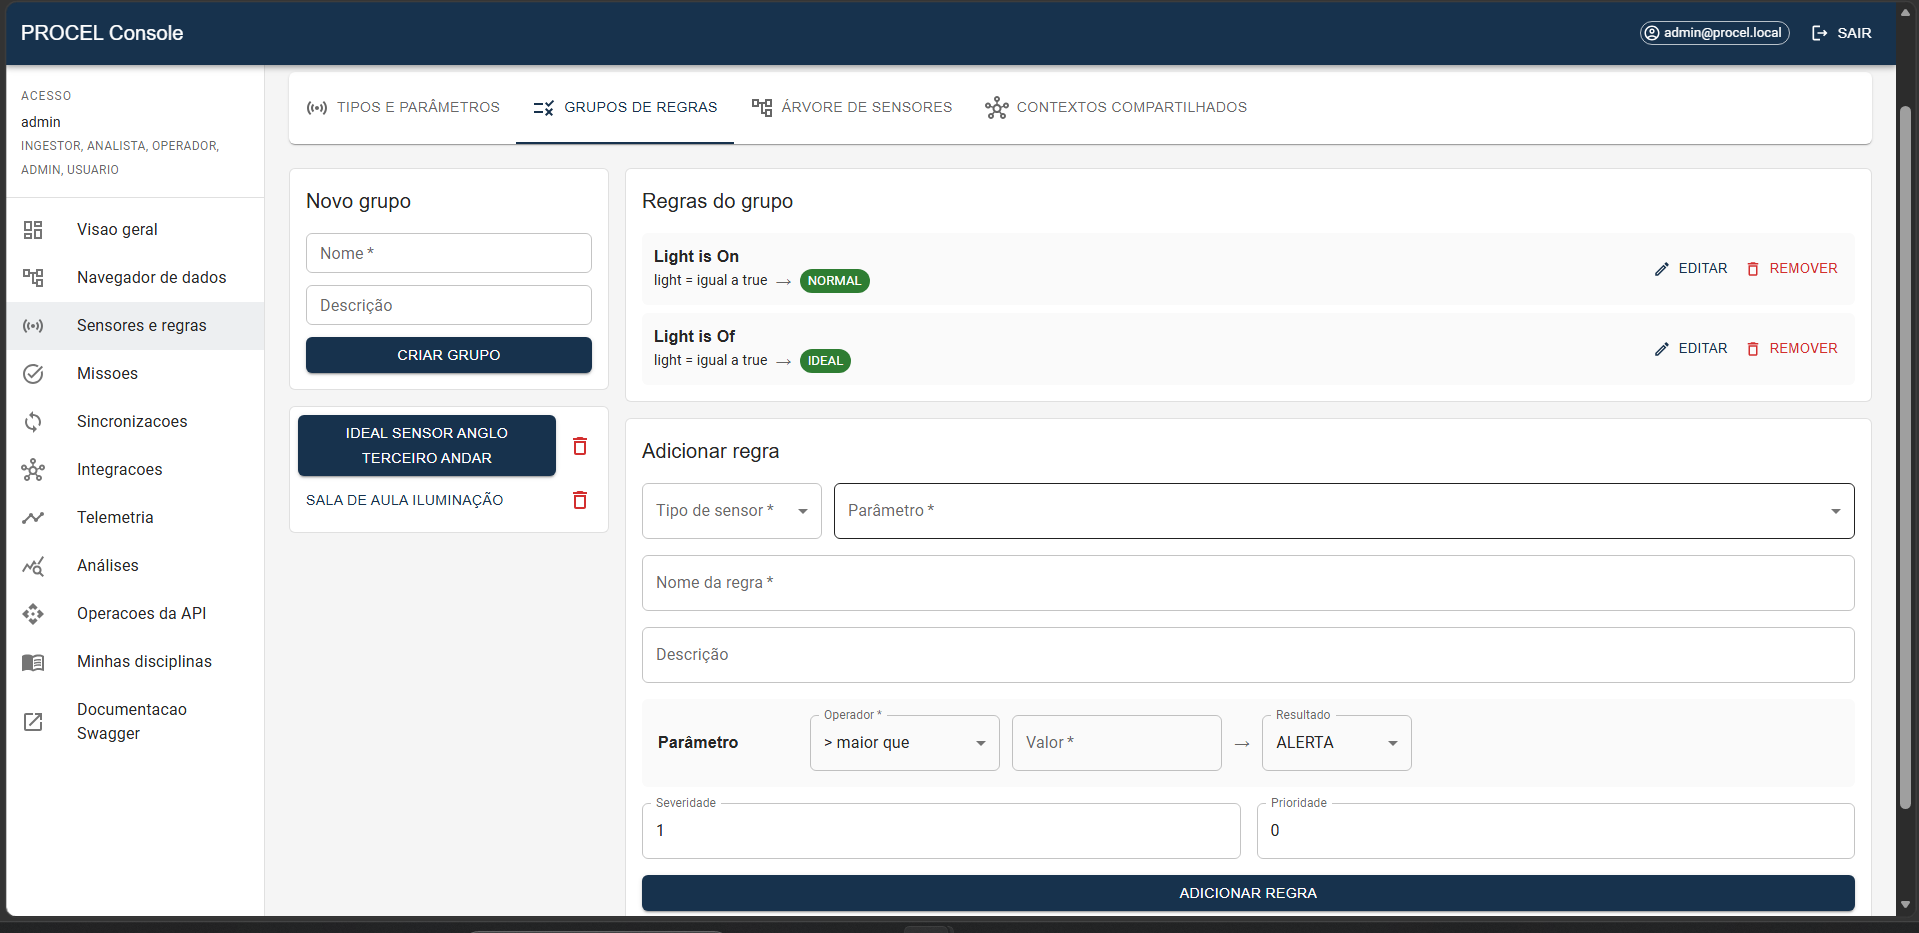
\includegraphics[width=\textwidth]{imagens/screenshots-do-PROCEL/Screenshot_4.png}
\caption*{Fonte: captura histórica do console fornecida pelo autor.}
\end{figure}
\begin{figure}[htbp]\centering
\caption{Registro histórico do console: configuração de missão e recompensa.}
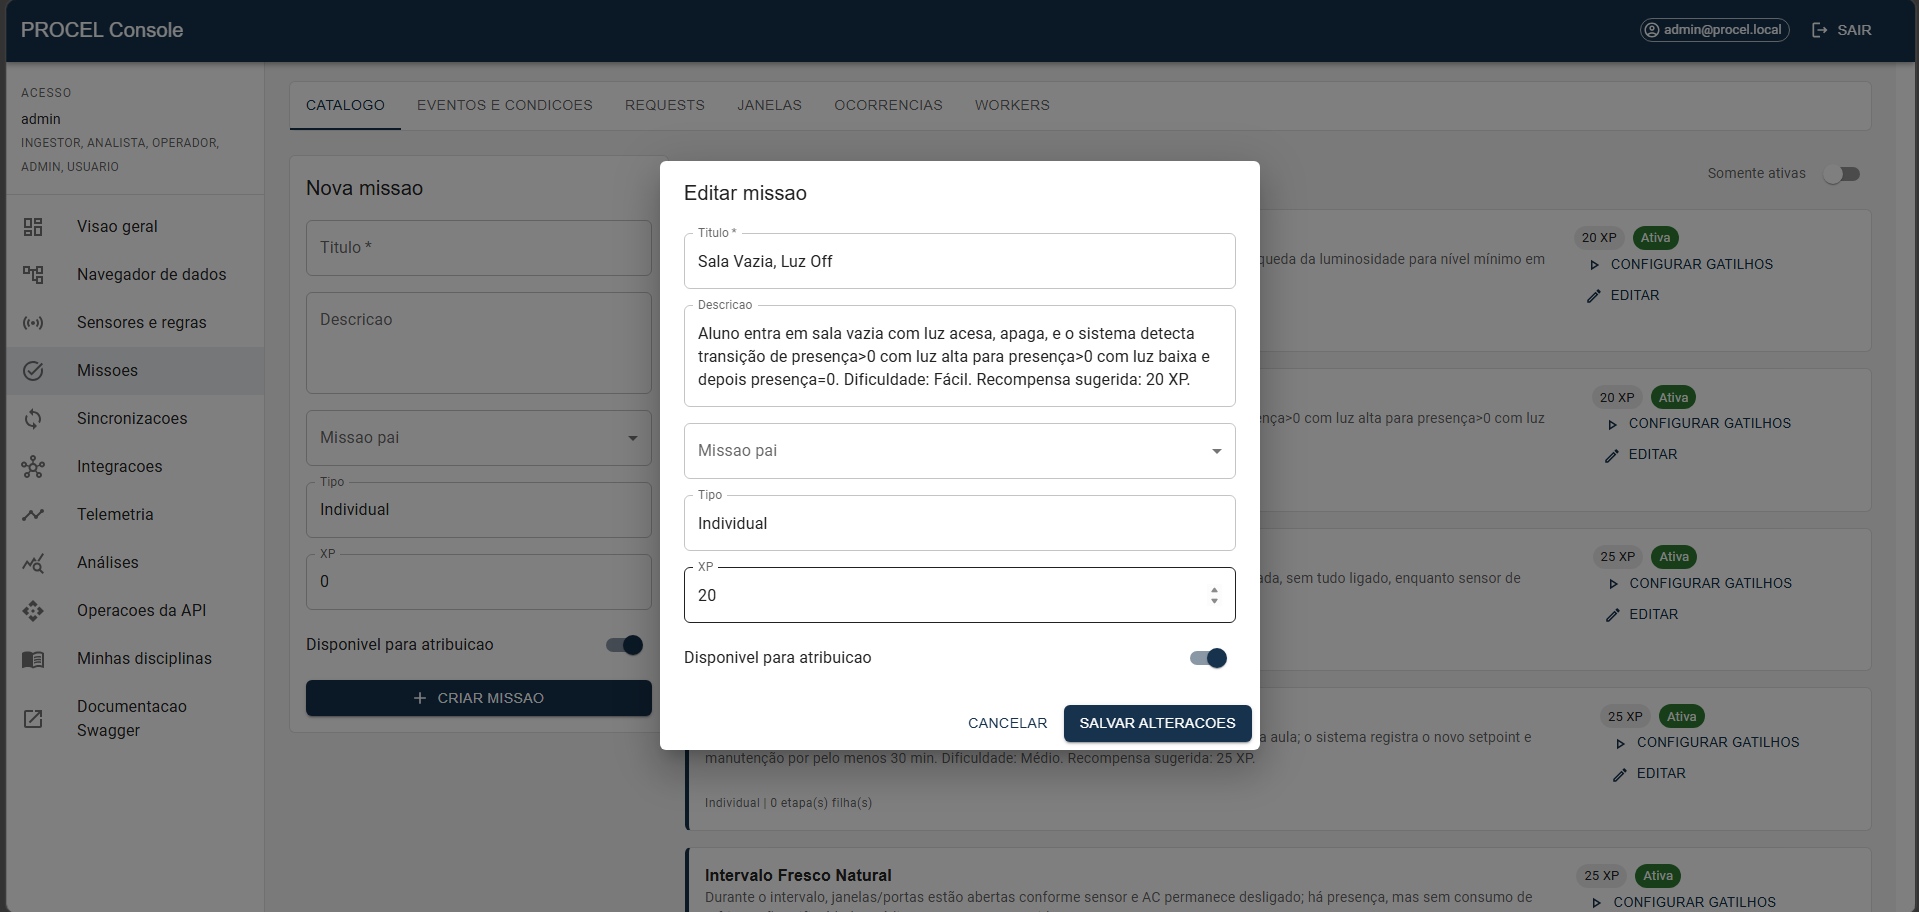
\includegraphics[width=\textwidth]{imagens/screenshots-do-PROCEL/Screenshot_7.png}
\caption*{Fonte: captura histórica do console fornecida pelo autor.}
\end{figure}
\clearpage
\bibliographystyle{abnt}
\bibliography{bibliografia}
\end{document}
